\chapter{Background}
\label{ch:background}

% Describe protocols and systems your work depends on.
% In almost all cases, this should contain a section on SCION.
In this chapter we give some background information needed to understand the following chapters.


\section{SCION}

SCION \cite{Perrig2022} is a clean-slate Internet architecture focused on scalability, control and isolation and is designed to provide security, flexibility, and performance improvements over the current Internet.
By putting the different autonomous systems (ASes) into groups called isolation domains (ISD), as seen in \cref{fig:scion_isd_architecture}, SCION can provide isolation between them.
Every ISD has some core ASes which administer the ISD, form the root of trust of the ISD and provide connectivity to other ISDs.
The configuration of an ISD is stored in a signed file called trust root configuration (TRC), which includes for example root certificates or policies.

\begin{figure}
    \centering
    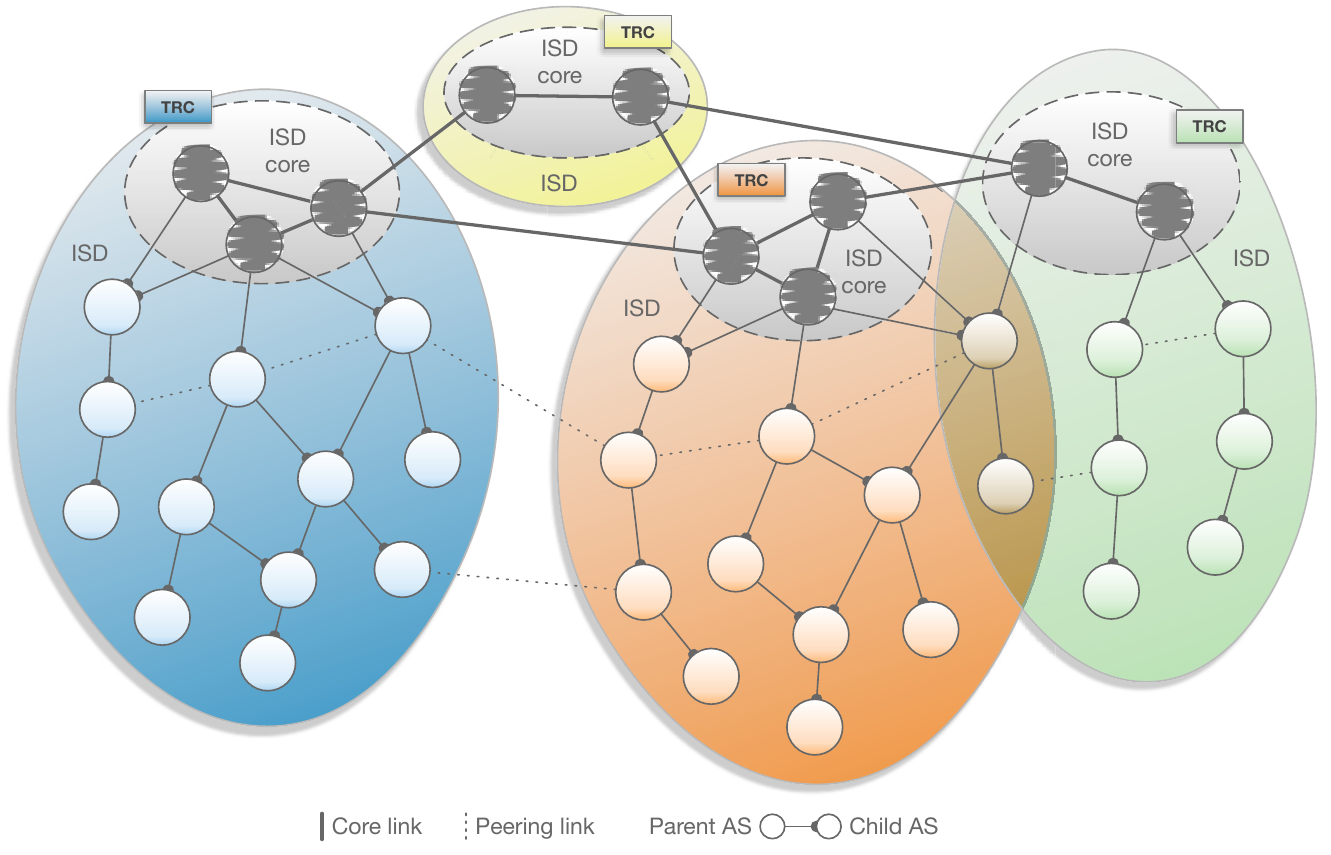
\includegraphics[width=0.75\textwidth]{figures/scion_isd_architecture.png}
    \caption{SCION Architecture with ISD and ASes. ASes are represented by circles. Figure taken form Chapter 2 of the SCION book \cite{Perrig2022}.}
    \label{fig:scion_isd_architecture}
\end{figure}

SCION offers users the ability to request and select the best paths to their desired destinations.
With the option to utilize multiple paths simultaneously, SCION empowers users with greater control and flexibility over their network traffic.






\section{Security Tools}


\subsection{Automatic Scanning Tools}
We mainly use Nessus and OpenVAS to scan and automatically detect potential vulnerabilities on the SCION devices.
The primary difference between Nessus and OpenVAS is that Nessus is a proprietary tool, while OpenVAS is open-source.
Both tools are free to use and can run unauthenticated as well as authenticated scans.
Since the authenticated scans use credentials to log in to the target device, they can gather more information about the device and provide more accurate results.
At the end of a scan, both tools generate reports that give a detailed overview of the vulnerabilities and weaknesses found on the scanned devices.




